\chapter{Architecture}
% TODO make diagrams more readable, discussion?

  The framework has been implemented as a 3-tier architecture. This allowed us to easily
  separate responsibilities and minimise coupling. The architecture focuses on allowing
  third party integrations easily with the use of the interceptor architectural pattern.
  To make it easy for clients to use the framework, a server is supplied which exposes
  a REST API. A pluggable adapter is used in order to allow the integration of other
  database systems which is an important feature.

  \section{Architectural Diagram}
  Clients can integrate on two levels. Clients can attach to dispatcher directly themselves or
  clients can register their modules. The framework then runs a flask REST server.
  A user can assemble their own pipeline via REST or a GUI. The framework in in charge or creating
  the supplied interceptors and attaching them to dispatchers and managing a pipeline on a thread.

  \section{Package Diagram}
    \begin{figure}[H]
        \hspace{-8em}
        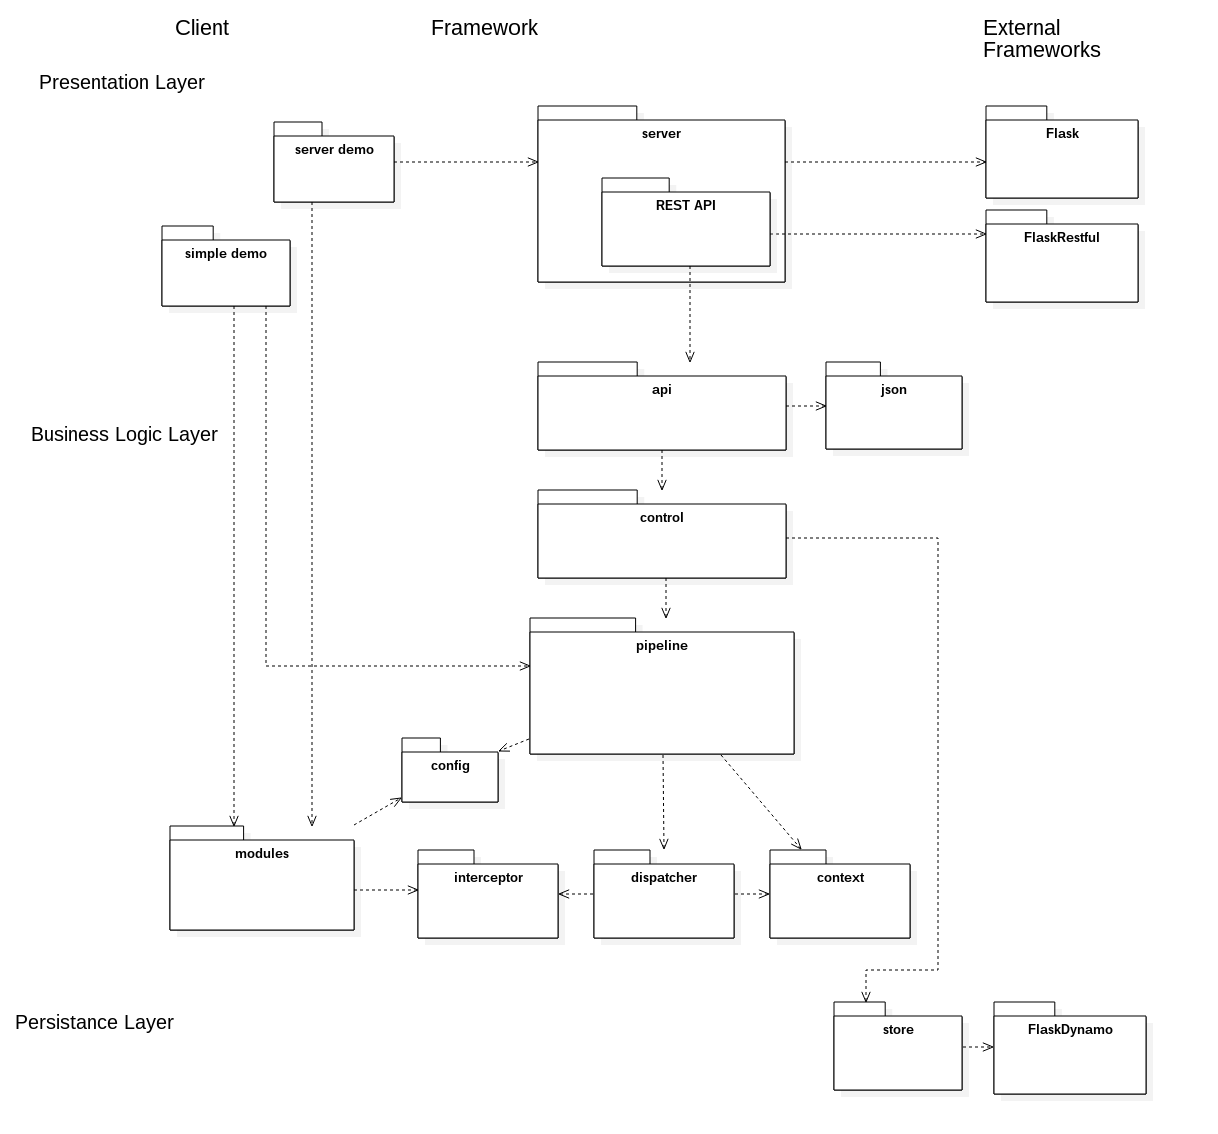
\includegraphics[width = 1.5\linewidth]{diagrams/architecture.png}
        \caption{Package Diagram}
        \label{fig:architecture_packages}
      \end{figure}

  \section{Class Diagram}
    \begin{figure}[H]
        \hspace{-4em}
        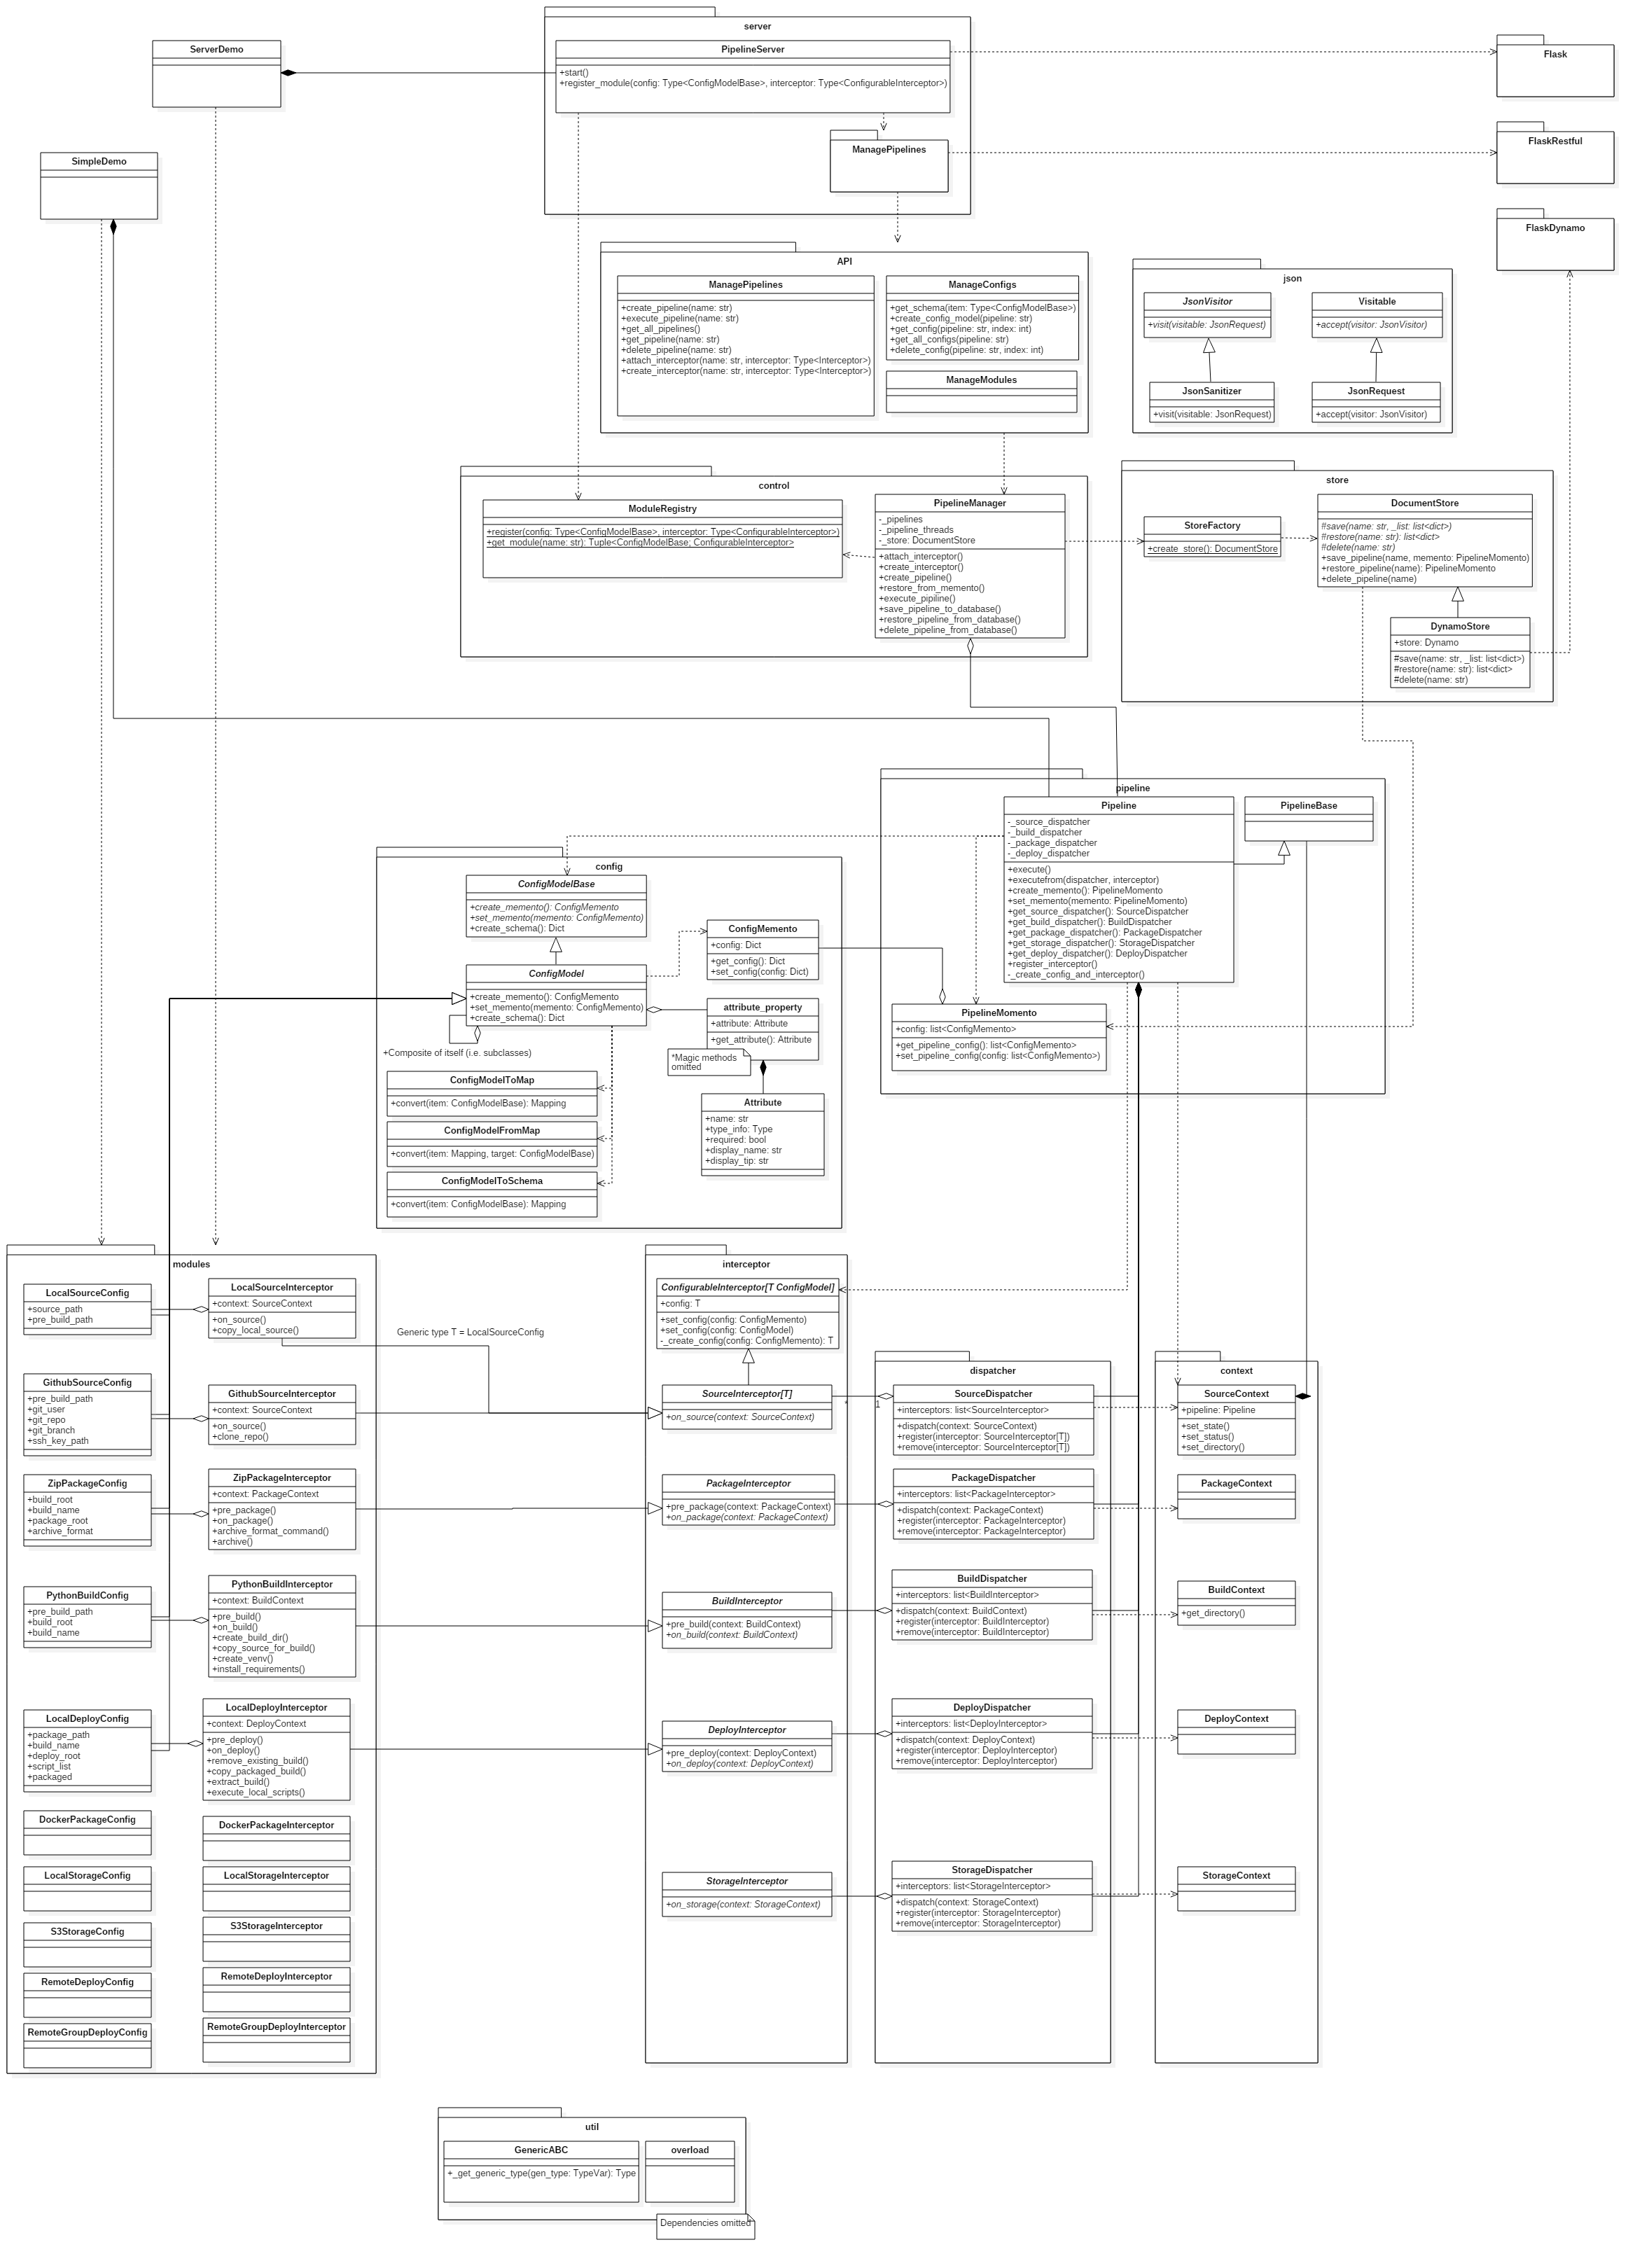
\includegraphics[width = 1.2\linewidth]{diagrams/architecture_classes.png}
        \caption{Architecture Class Diagram}
        \label{fig:architecture_classes}
      \end{figure}

    \section{Class Diagram Fragments}
    TODO


   \section{Sequence Diagram}
	   \begin{figure}[H]
	   	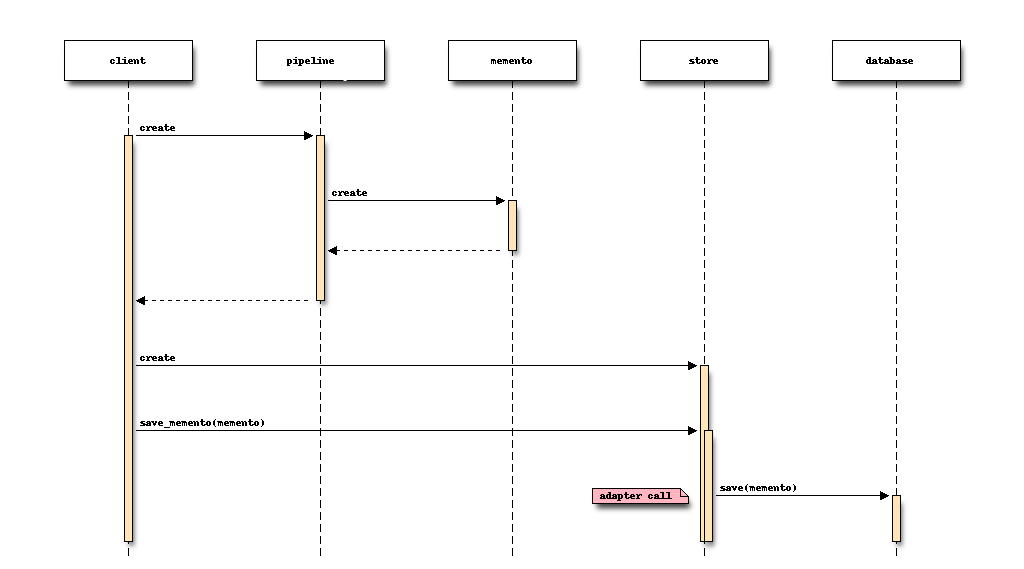
\includegraphics[width = 1.2\linewidth]{diagrams/sequence_diagram.png}
	   	\caption{Pluggable Adapter Sequence Diagram}
	   \end{figure}

TODO structural diagram
